\apendice{Documentación técnica de programación}

\section{Introducción}
Hay una serie de elementos relativos al proyecto que no tiene que ver estrictamente con el desarrollo, pero que pueden ser útiles conocer (tales como la estructura de ficheros, la importación y exportación del proyecto o la pruebas de sistema). Se explicarán a continuación. 

\section{Estructura de directorios}
Se va a comentar la estructura de ficheros del repositorio de GitHub que contiene todos los materiales relativos al proyecto.

\begin{itemize}
\item
/: Directorio raíz del repositorio.
\item
/docs: Directorio que contiene todos los ficheros relativos a la documentación.
\item
/docs/Latex: Carpeta con todos los ficheros necesarios para la generación de la memoria y los anexos con Latex.
\item
/docs/Latex/img: Contiene todas las imágenes que aparecerán el los ficheros generado en Latex.
\item
/docs/Latex/tex: Contiene los ficheros de Latex secundarios que utilizarán los principales para generar la memoria y los anexos.
\item
/game: Contiene la solución de Visual Studio con el código relativo al vidojuego desarrollado.
\item
/game/Assets: Contiene todos los ficheros de código en C\# y en formatos especializados de Unity necesarios para que Unity pueda exportar el juego correctamente.
\item
/game/Assets/Audio: Ficheros de audio del proyecto.
\item
/game/Assets/Character: Elementos estéticos exclusivos del Player.
\item
/game/Assets/Character/Animations: Animaciones que provee Platformer Microgame utilizadas en el Player.
\item
/game/Assets/Character/Sprites: Sprites del Player.
\item
/game/Assets/Environment: Sprites utilizados para crear los mapas de los niveles jugables.
\item
/game/Assets/ModAssets: Elementos estéticos extra que provee Platformer Microgame para ofrecer más variedad estética.
\item
/game/Assets/Prefabs: Contiene todos los prefabs del proyecto.
\item
/game/Assets/Scenes: Contiene todas las escenas que conforman el proyecto.
\item
/game/Assets/Scripts: Ficheros de C\# utilizados en el proyecto.
\item
/game/Assets/Scripts/Animation: Ficheros de C\# utilizados en el proyecto relativos a la animación de sprites.
\item
/game/Assets/Scripts/Core: Ficheros de C\# utilizados en el proyecto. Contiene las clases encargadas del funcionamiento básico de los niveles.
\item
/game/Assets/Scripts/Gameplay: Ficheros de C\# utilizados en el proyecto. Contiene las clases que son eventos de Simulation.
\item
/game/Assets/Scripts/GizmosUI: Ficheros de C\# utilizados en el proyecto. Contiene las clases utilizadas para mostrar los Gizmos en el editor.
\item
/game/Assets/Scripts/Mechanics: Ficheros de C\# utilizados en el proyecto. Contiene las clases que implementa las mecánicas del juego.
\item
/game/Assets/Scripts/Model: Ficheros de C\# utilizados en el proyecto. Contiene una clase con las variables que se consultarán durante los niveles.
\item
/game/Assets/Scripts/Sound: Ficheros de C\# utilizados en el proyecto. Contiene las clases encargadas de gestionar el audio.
\item
/game/Assets/Scripts/UI: Ficheros de C\# utilizados en el proyecto. Contiene todas las clases relativas a la interfaz de usuario.
\item
/game/Assets/Scripts/View: Ficheros de C\# utilizados en el proyecto. Contiene clases que ofrecen comportamientos que afectan de forma especial a como debería verse un objeto.
\item
/game/Assets/Sprites: Sprites del proyecto que no pertenecen a Platformer Microgame.
\item
/game/Assets/Scripts: Elementos usados para generar mapas mediante la herramienta Tilemap de Unity.
\item
/executables: Contiene los ficheros comprimidos con el producto final. Hay un fichero comprimido para la versión del videojuego para Windows, otra para Linux y otra para WebGL.
\end{itemize}

\section{Manual del programador}
\subsection{Ventanas de Unity}
Se van a listar a continuación una serie de ventanas del editor de Unity y se explicará su propósito.

\subsubsection{Console}
Consola interna de Unity que mostrará los print realizados por las clases Monobehaviour y errores y warnings de compilación y ejecución.

\clearpage
\begin{figure}[h]
\centering
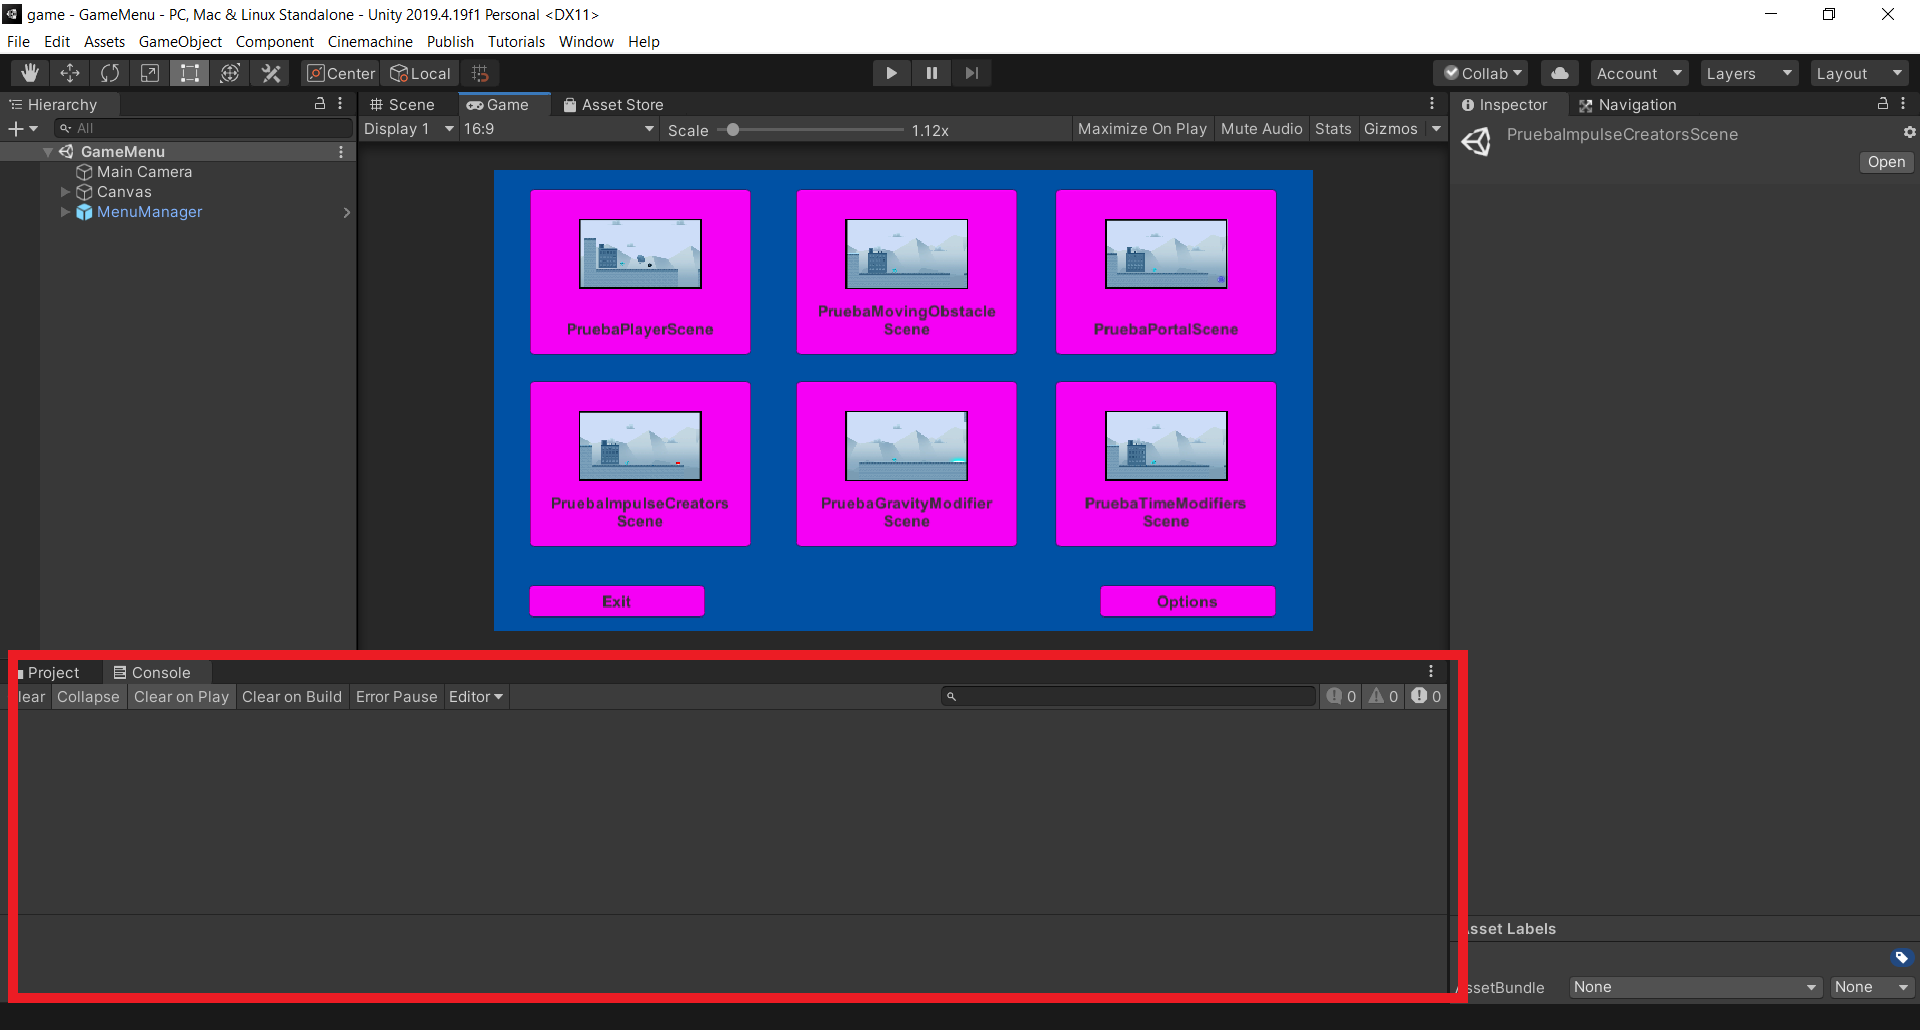
\includegraphics[scale=0.3]{Anexos/Anexo_D/Consola_Unity}
\caption{Consola de Unity}
\end{figure}

\subsubsection{Project}
Ventana que muestra todo el sistema de ficheros del proyecto que se está desarrollando.

\begin{figure}[h]
\centering
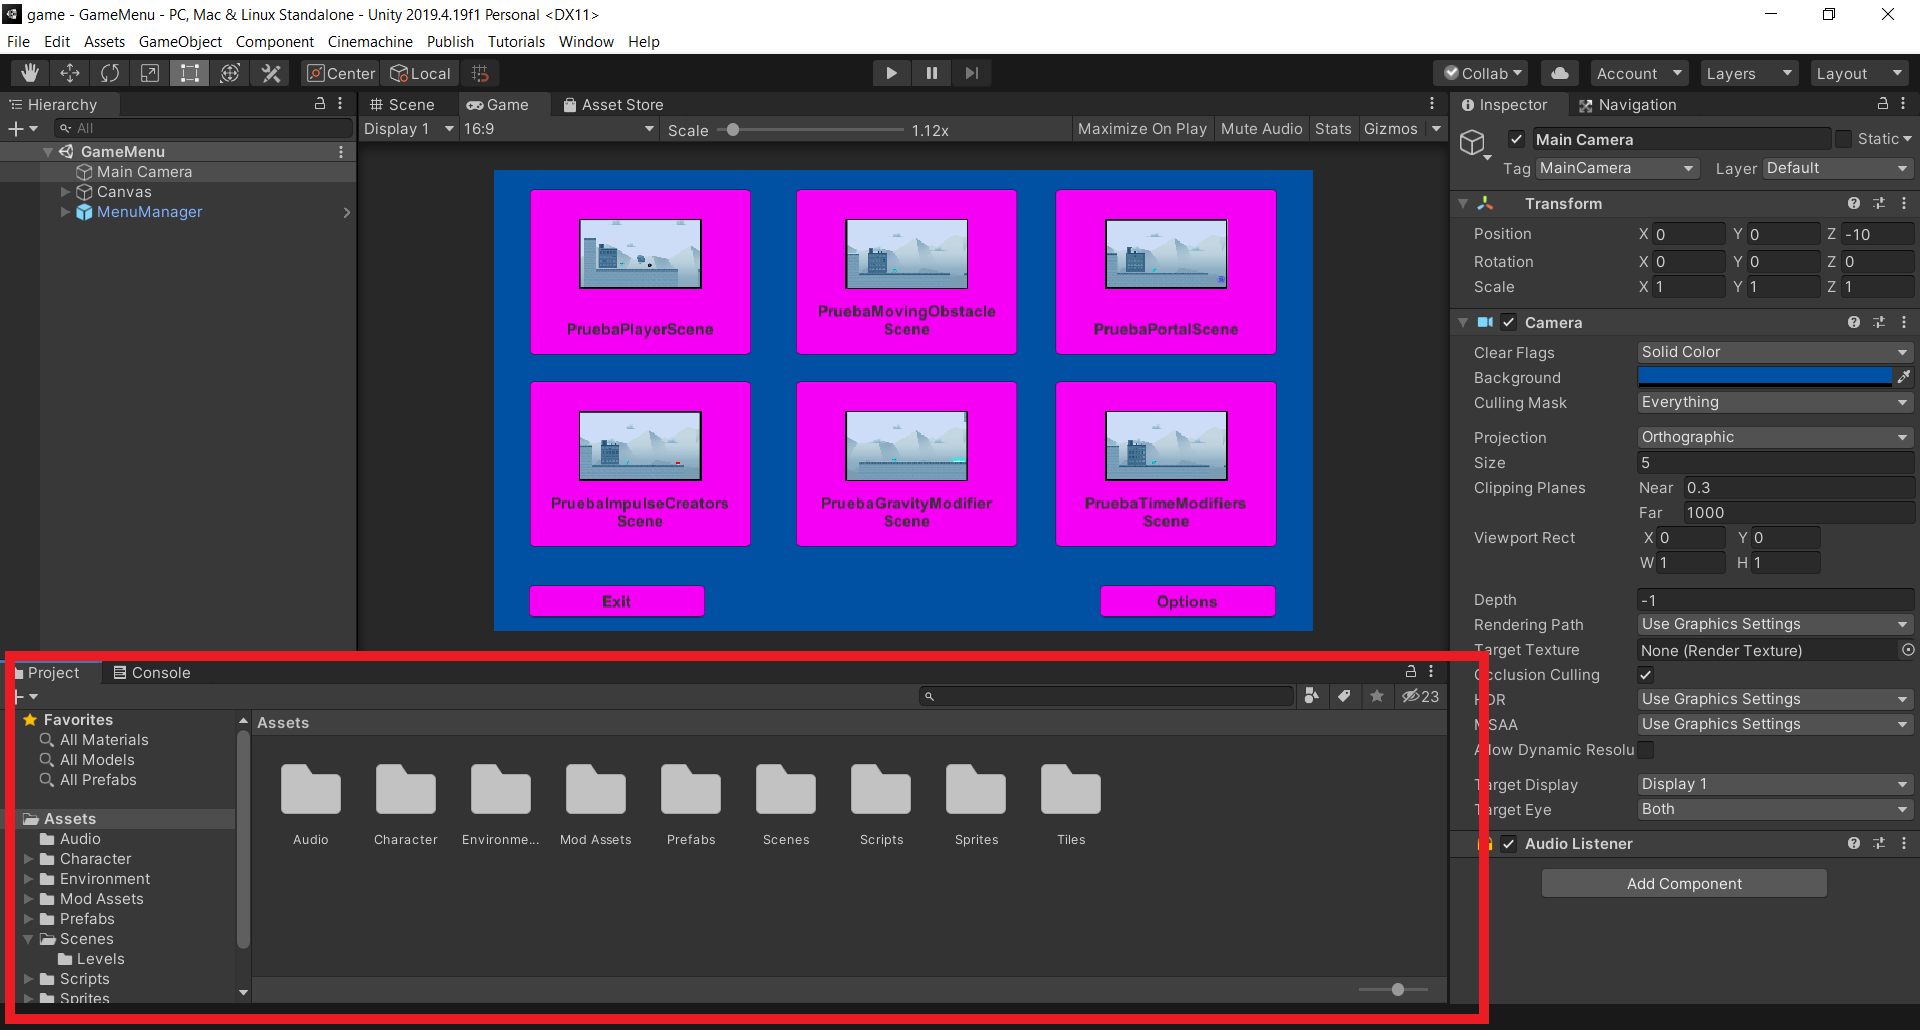
\includegraphics[scale=0.2]{Anexos/Anexo_D/Project}
\caption{Vetana ''Project'' de Unity}
\end{figure}
\clearpage

\subsubsection{Hierarchy}
Ventana que muestra los elementos que componen la escena y las dependencias padre-hijo entre estos.

\begin{figure}[h]
\centering
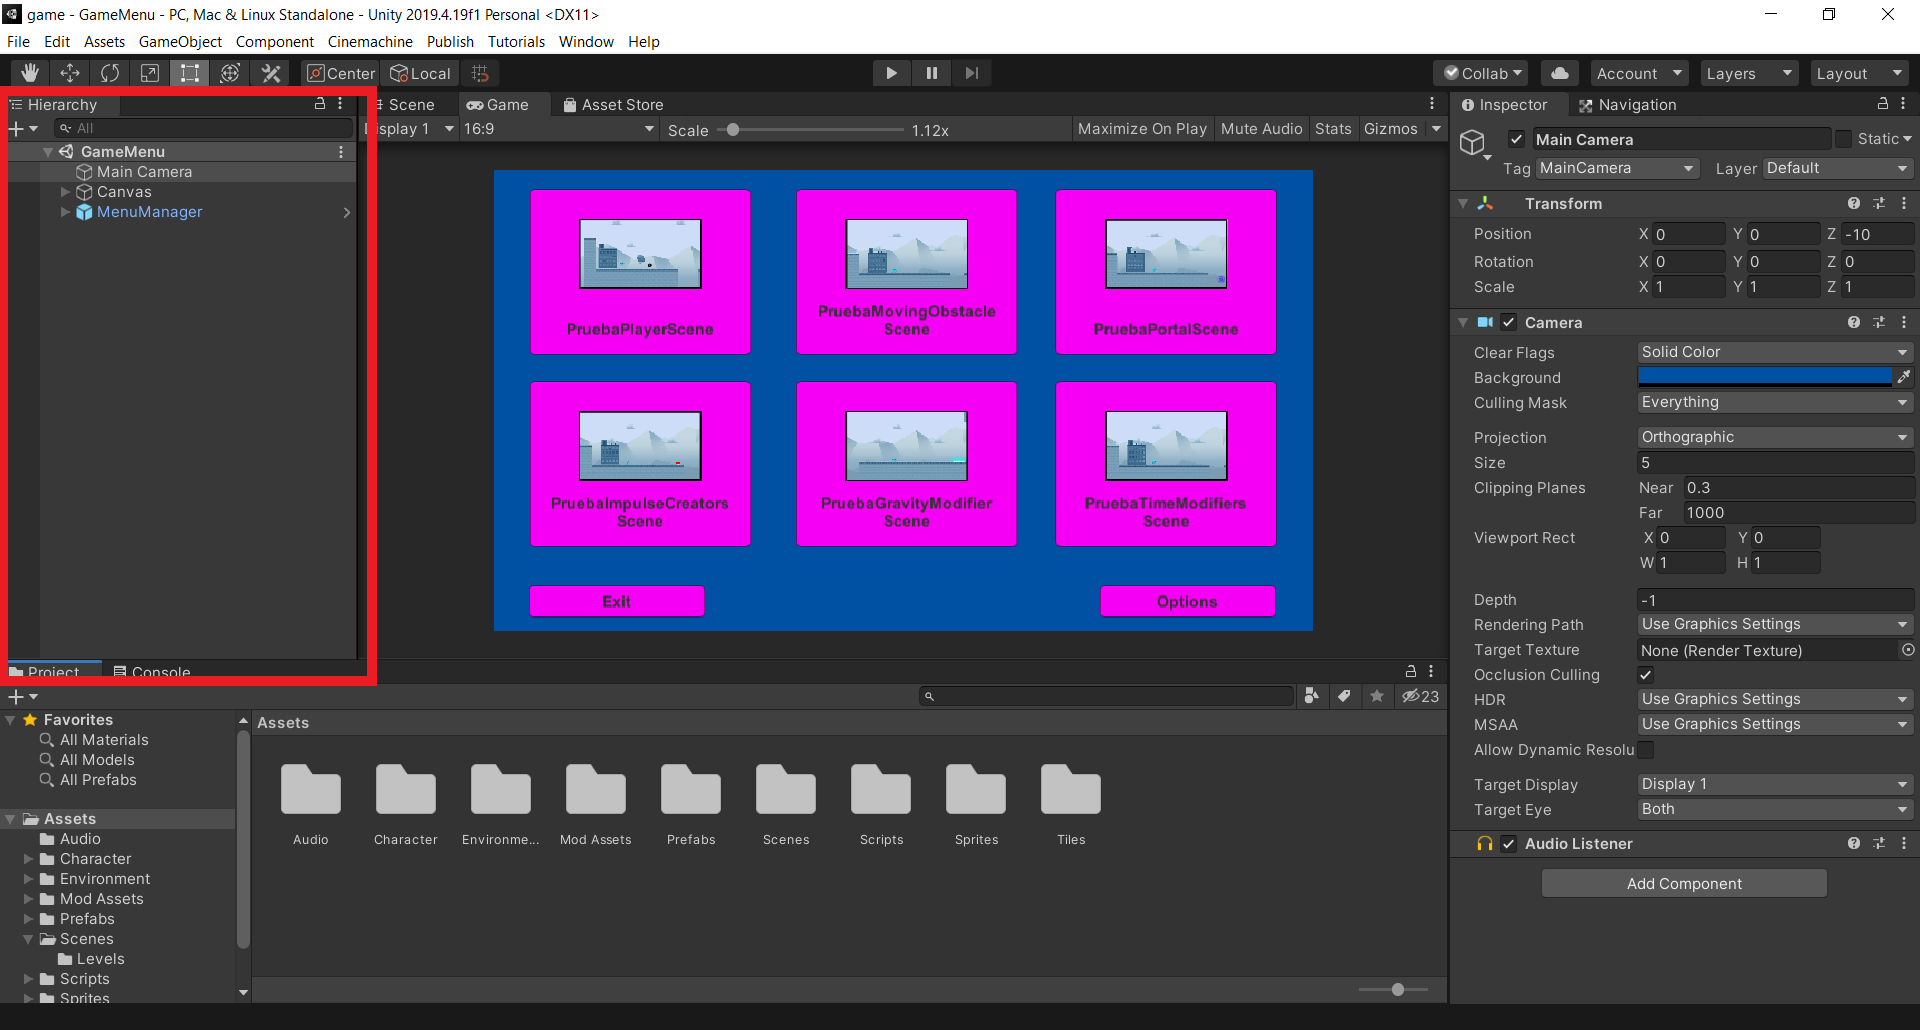
\includegraphics[scale=0.3]{Anexos/Anexo_D/Hierarchy}
\caption{Ventana ''Hierarchy'' de Unity}
\end{figure}

Estos elementos serán distintos para cada escena. Sin embargo en los niveles jugables tendrán una serie de elementos comunes:
\begin{itemize}
\item
MainCamera: Cámara encargada de mostrar por pantalla lo que el jugador debe ver.
\item
OptionsMenuCanvas: Estructura de objetos que conformarán el menú de pausa.
\item
GameController: Objeto encargado de que el juego mantenga un estado estable. Tiene un objeto hijo que es un reproductor de música.
\item
SpawnPoint: Punto de aparición del Player. También reaparecerá en este punto tras morir.
\item
Player: Avatar que controlará el jugador.
\item
CineachineConfiner: La cámara no se podrá desplazar más allá de los límites marcados por este objeto.
\item
CM vcam1: Objeto encargado del control del movimiento de la cámara.
\item
Grid: Contiene los Tilemaps que construyen el nivel. Tiene 4 objetos hijos: FarBackgroundTilemap para elementos muy alejados del nivel (montañas), BackgroundTilemap para elementos alejados del nivel (nubes), LevelTilemap para elementos que forman parte del nivel y se espera poder interactuar con ellos (suelos y paredes) y ElementsTilemap para elementos que forman parte del nivel, pero son puramente estéticos (árboles y edificios).
\item
Zones: zonas relevantes del nivel. Podrán ser de tres tipos: muros o suelos, zonas de muerte y zonas de victoria.
\end{itemize}

\subsubsection{Inspector del Objeto}
Ventana que muestra la información y ajustes de los componentes que conforman un GameObject seleccionado.

\begin{figure}[h]
\centering
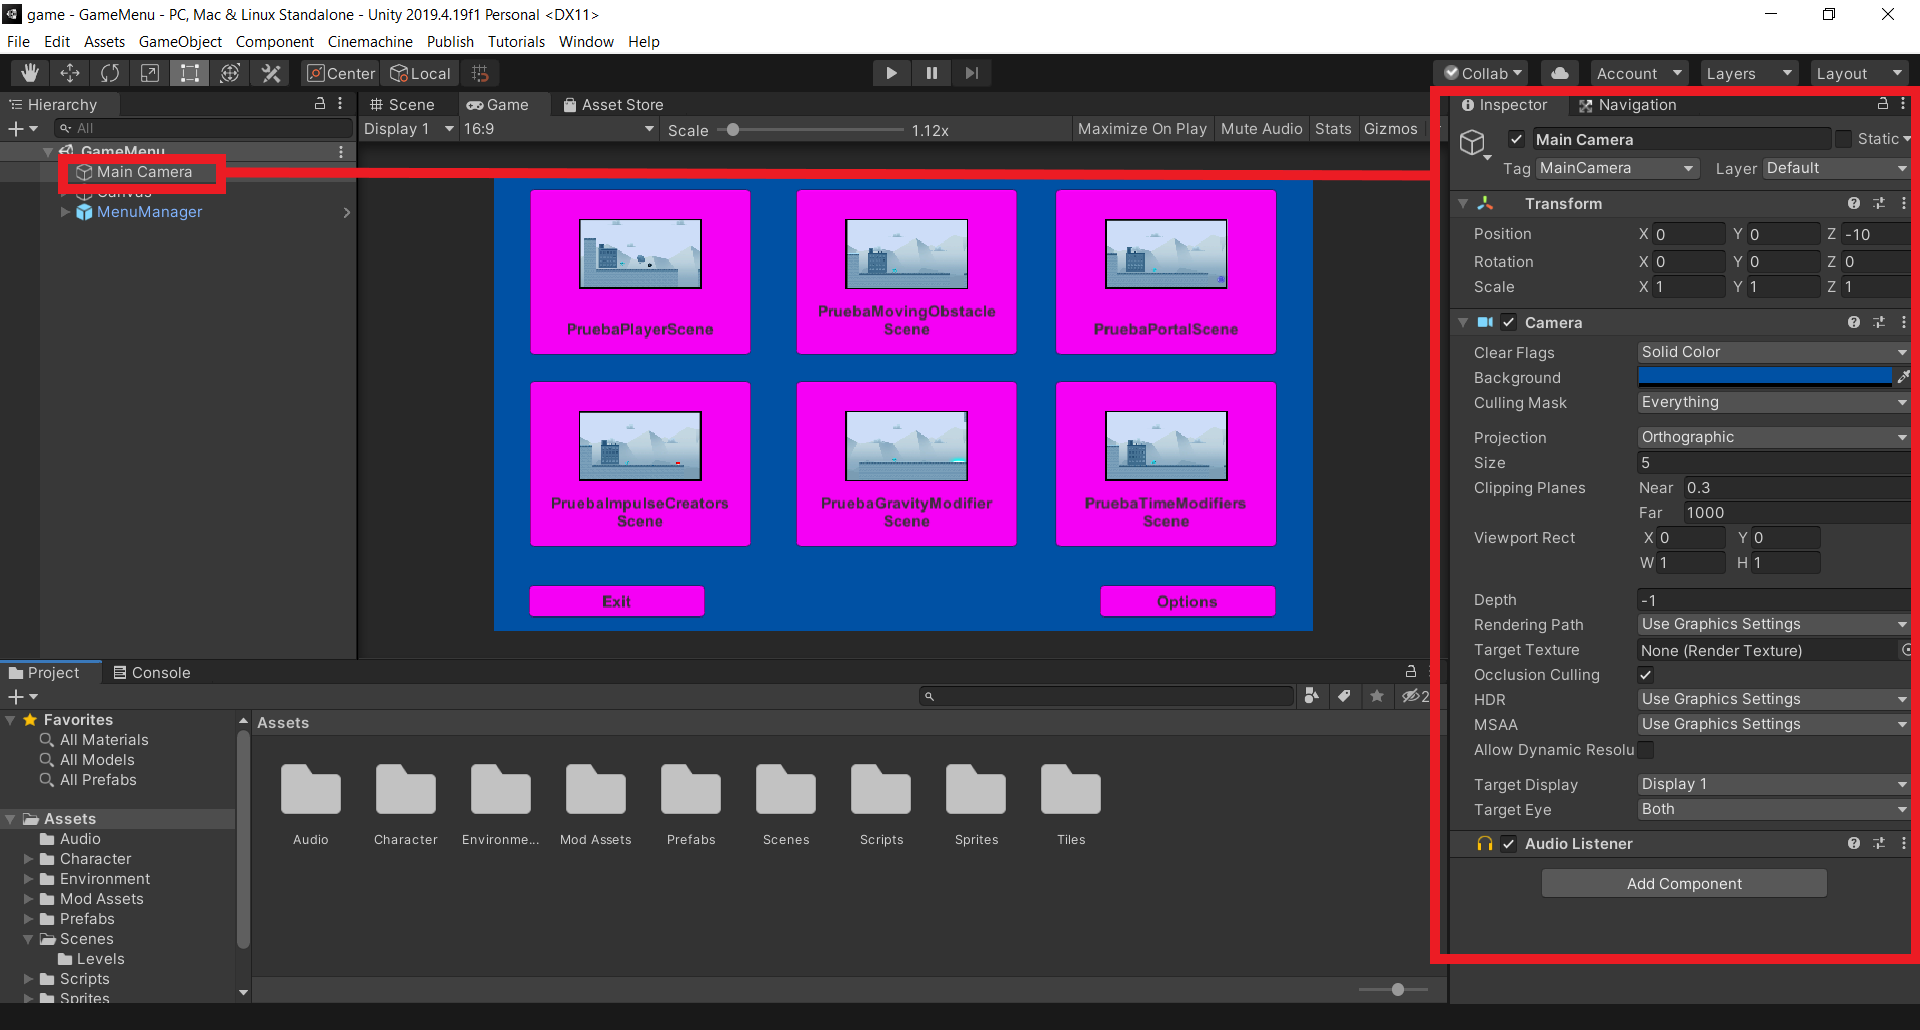
\includegraphics[scale=0.3]{Anexos/Anexo_D/Info}
\caption{Información asociada al GameObject Main Camera}
\end{figure}

\subsubsection{Game}
Ventana que muestra como se verá el juego en ejecución. Si se ejecuta el proyecto mostrará como se verá el juego en tiempo de ejecución actualizándose en cada frame.

\begin{figure}[h]
\centering
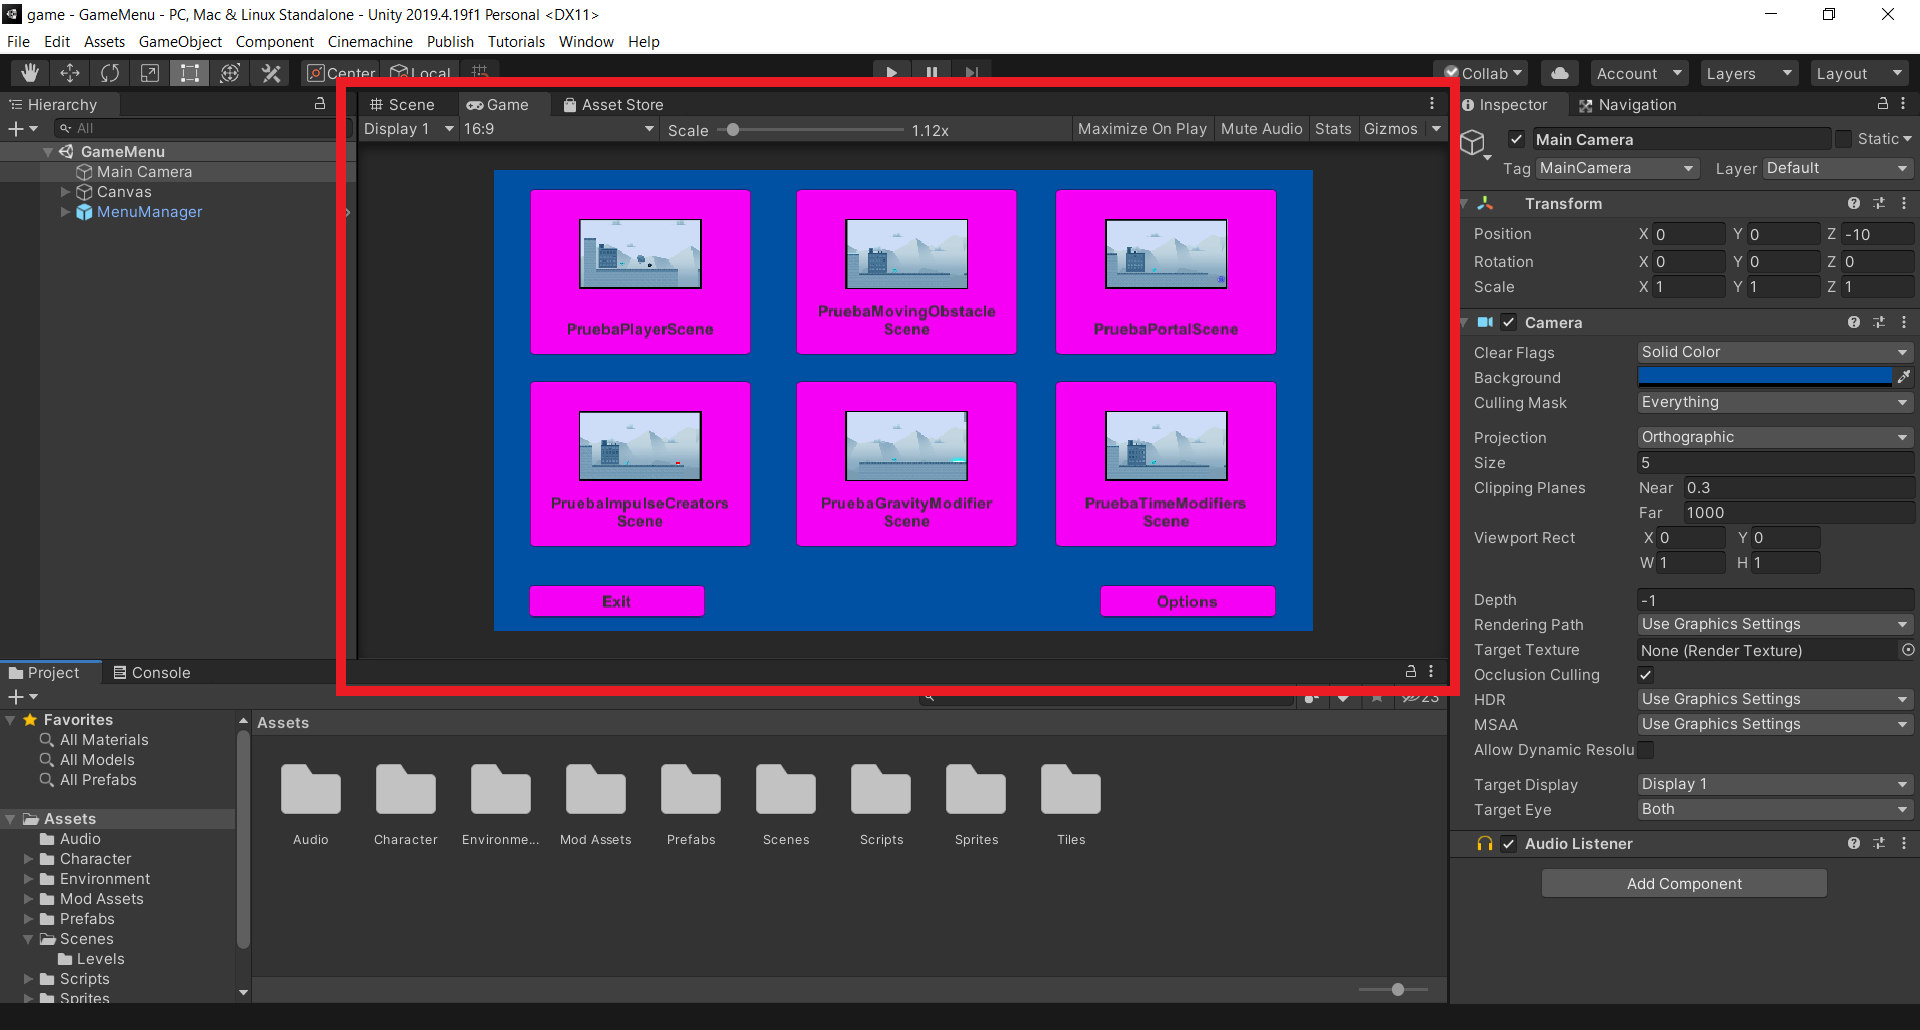
\includegraphics[scale=0.3]{Anexos/Anexo_D/Game}
\caption{Vetana ''Game'' de Unity}
\end{figure}

\subsubsection{Scene}
Ventana que muestra como visualmente donde estaría cada objeto de ''Hierarchy'' en un entorno físico. Como el desarrollo es de un Plataformas 2D se mostrará el entorno físico en dos dimensiones, pero también es posible generar el entorno en 3D (en realidad el entorno generado es 3D, pero con una colocación de cámara que simula ser 2D).

\clearpage
\begin{figure}[h]
\centering
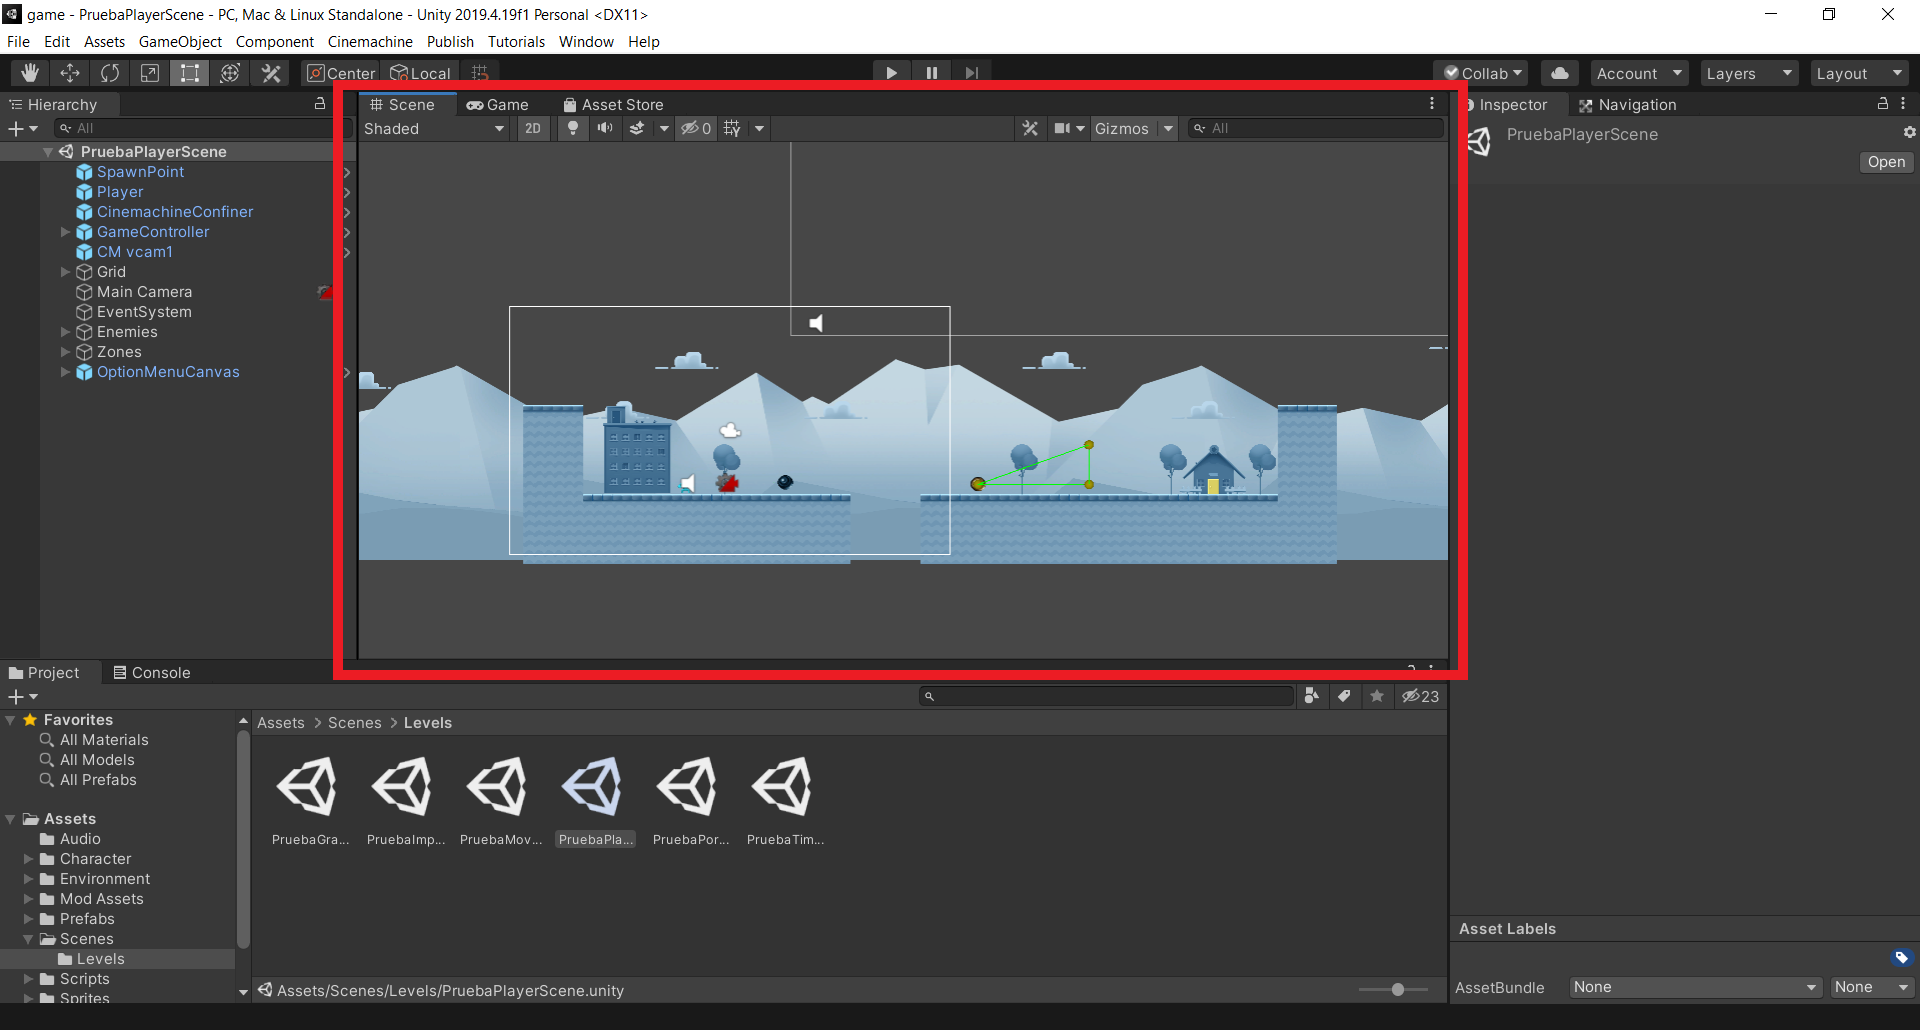
\includegraphics[scale=0.3]{Anexos/Anexo_D/Scene}
\caption{Ventana ''Scene'' de Unity}
\end{figure}

\subsection{Importación del proyecto}
El proyecto de Unity está en la carpeta game del repositorio de Github y será necesario guardado en el ordenador en el que se desee importar para poder importarlo.
Para importar el proyecto lo único que hay que hacer es, en el apartado ''Proyects'' del Unity Hub pulsar el botón de ''ADD''.

\begin{figure}[h]
\centering
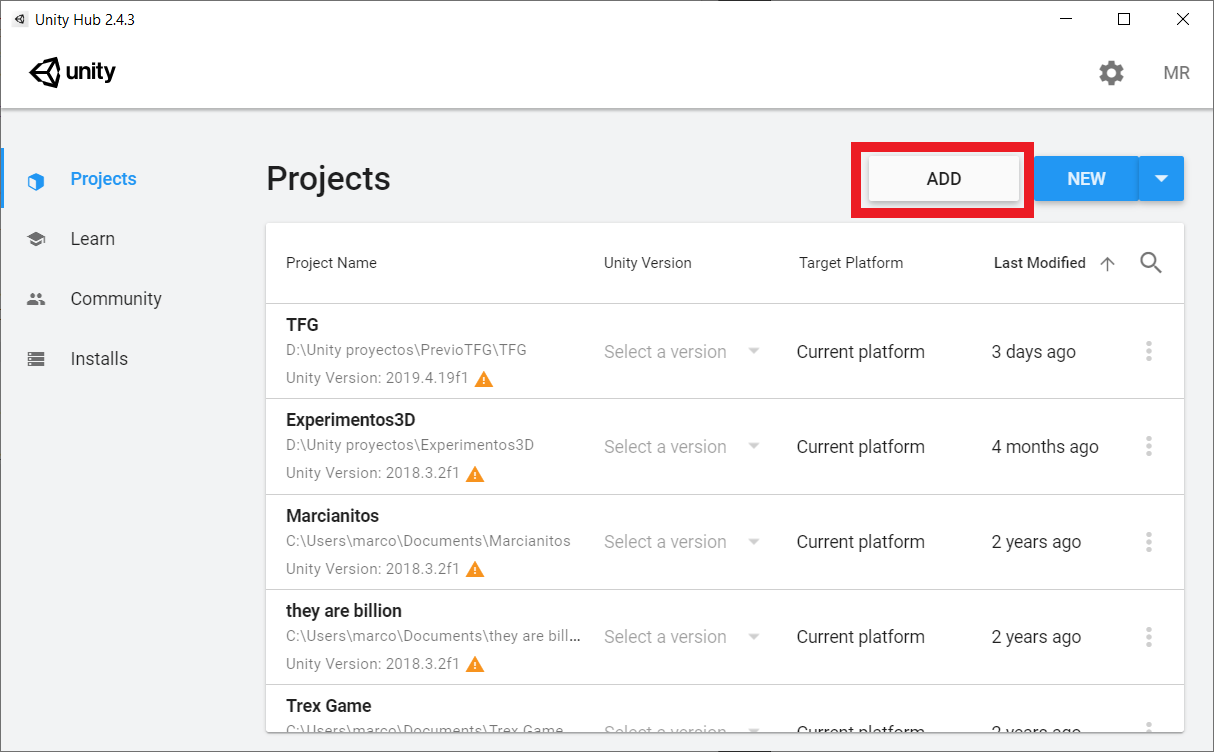
\includegraphics[scale=0.2]{Anexos/Anexo_D/Prujects_add}
\caption{Importación del proyecto de Unity desde Unity Hub}
\end{figure}
\clearpage

Después de pulsar el botón se pedirá una ruta. Introducir la ruta donde esté guardada la carpeta game del repositorio de GitHub.

\begin{figure}[h]
\centering
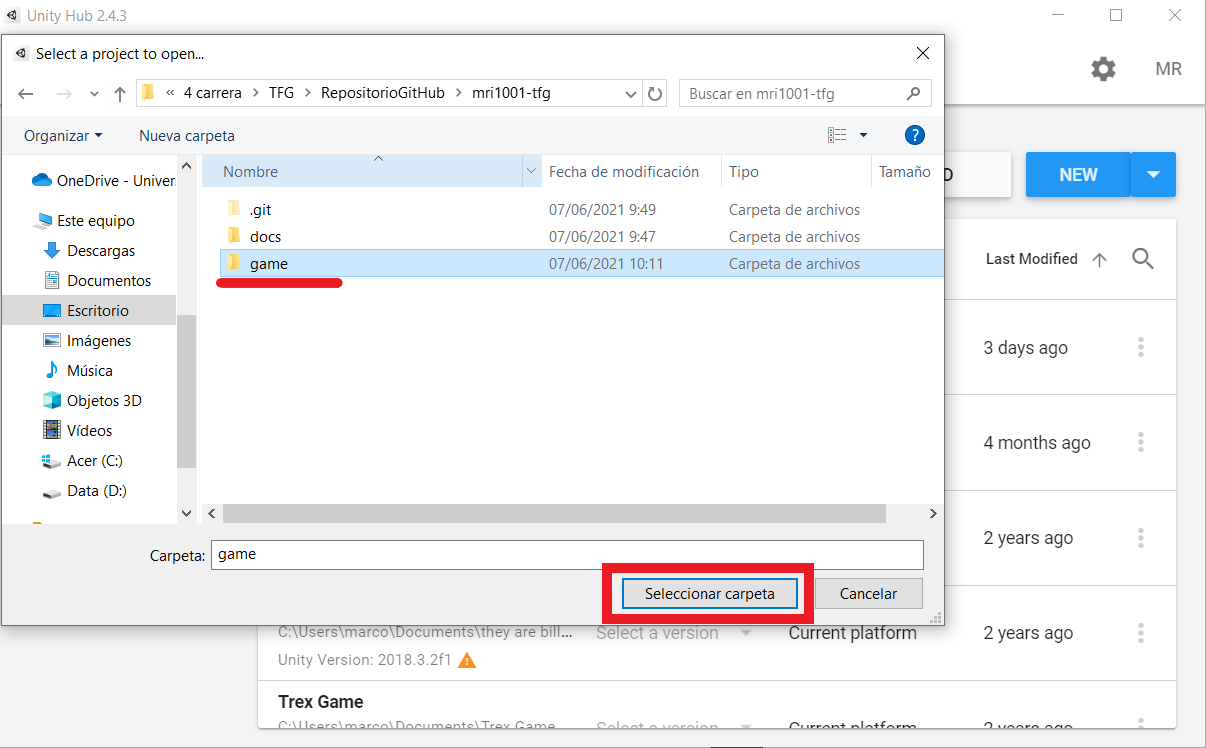
\includegraphics[scale=0.3]{Anexos/Anexo_D/Project_ruta}
\caption{Selección ruta del proyecto de Unity desde Unity Hub}
\end{figure}

Se añadirá a la lista de proyectos de Unity el proyecto importado y ya se podrá acceder a él.

\begin{figure}[h]
\centering
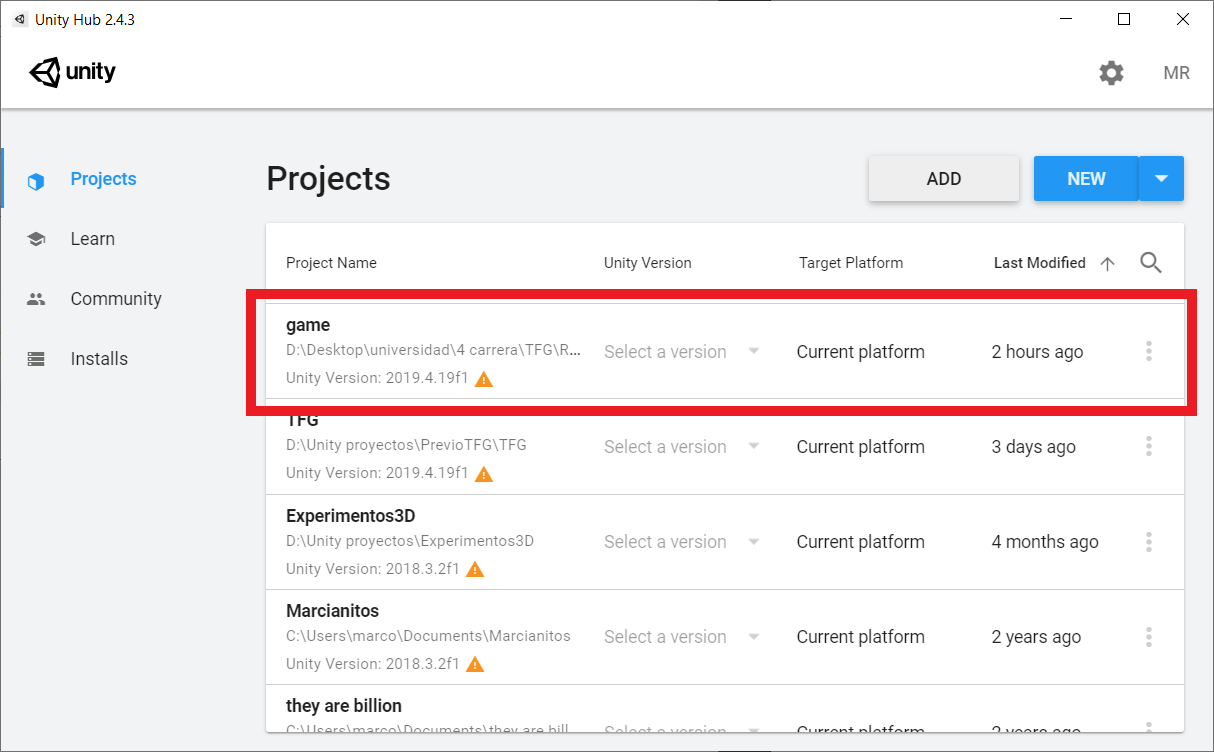
\includegraphics[scale=0.3]{Anexos/Anexo_D/Project_creado}
\caption{Proyecto importado correctamente}
\end{figure}

Al abrir el proyecto por primera vez saldrá una escena por defecto vacía. Con seleccionar cualquier otra escena será suficiente para que desaparezca esa escena y el funcionamiento sea el normal.

\subsection{Exportación del proyecto}
Para exportar el proyecto y generar el videojuego con su correspondiente ejecutable solo es necesario ir a la pestaña de File → Build Settings de la barra de herramientas superior del editor de Unity.\\
Al hacerlo aparecerá la siguiente ventana:

\begin{figure}[h]
\centering
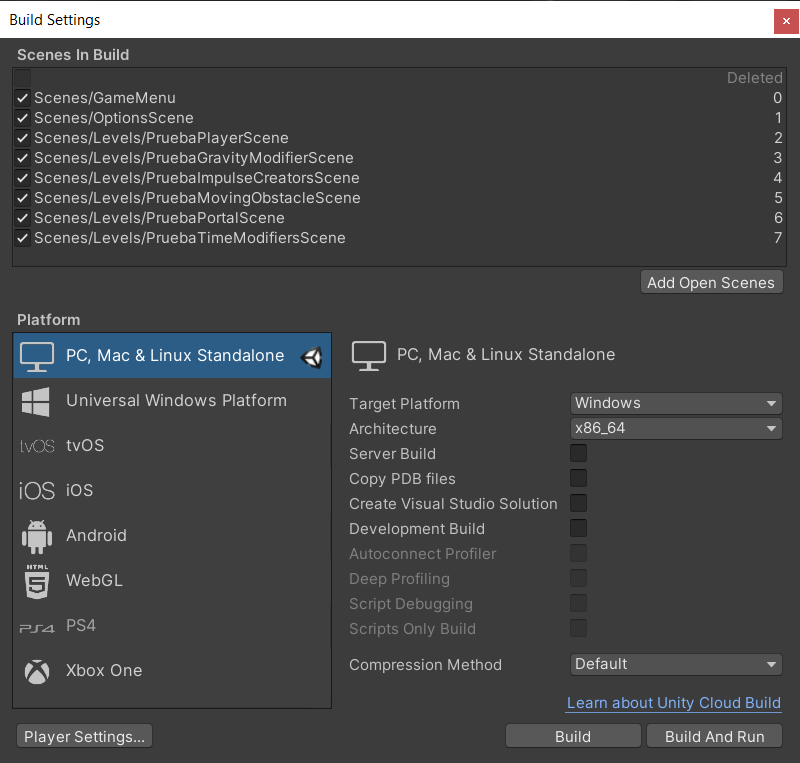
\includegraphics[scale=0.3]{Anexos/Anexo_D/Build}
\caption{Ventana de construcción del juego}
\end{figure}

Esta ventana da la opción de elegir a que sistema operativo y plataforma exportarlo entre otras opciones.

\begin{figure}[h]
\centering
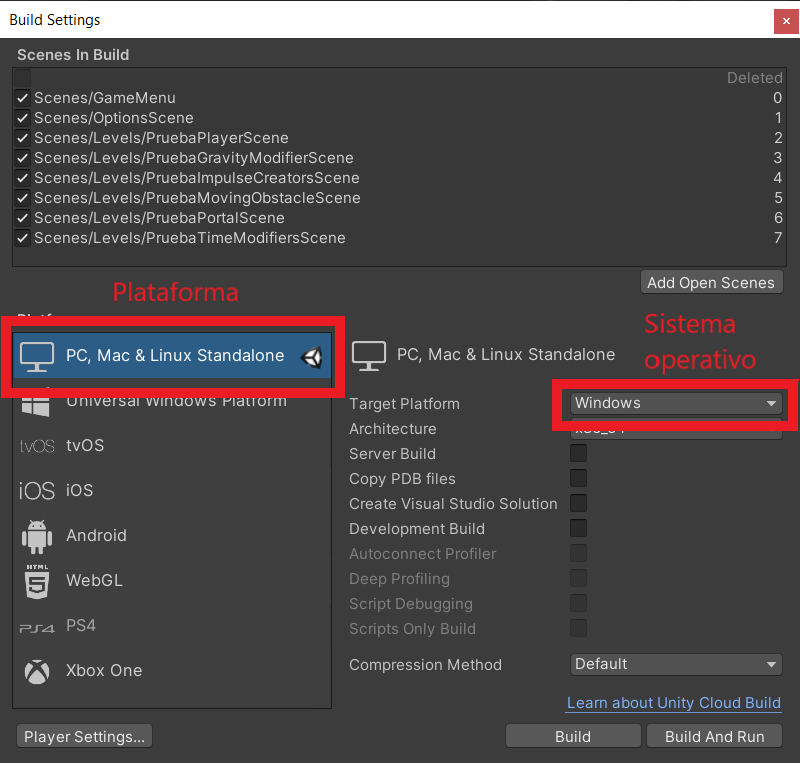
\includegraphics[scale=0.3]{Anexos/Anexo_D/Plataforma}
\caption{Seleción de plataforma y Sistema operativo}
\end{figure}

Es muy importante que el tick esté en todas las escenas a las que se desee transicionar para poder viajar a ellas.

\begin{figure}[h]
\centering
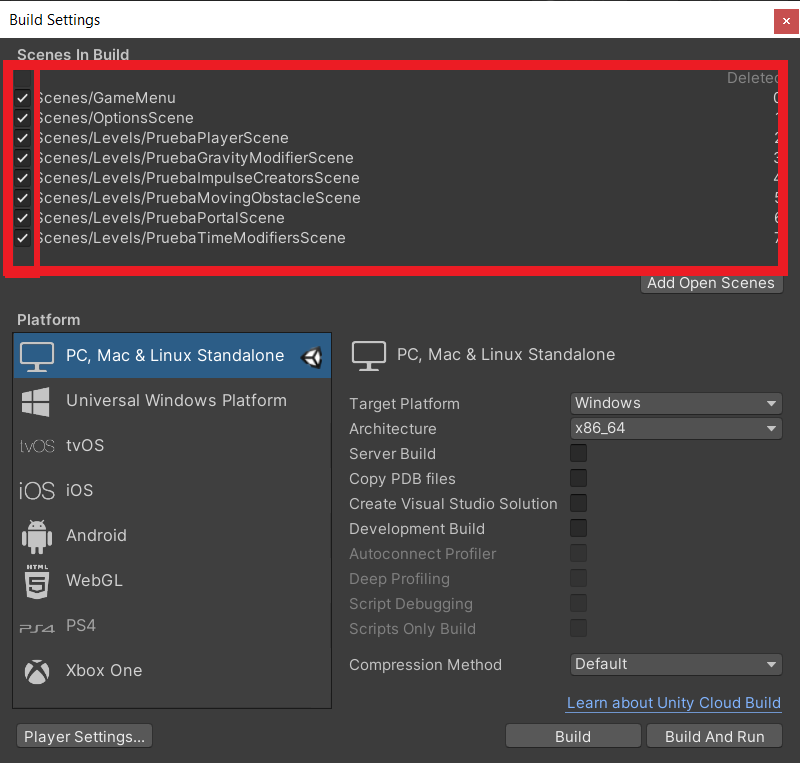
\includegraphics[scale=0.3]{Anexos/Anexo_D/Scenes}
\caption{Escenas seleccionadas para exportar}
\end{figure}

Una vez hecha esta comprobación se puede dar al botón ''Build'' para comenzar la exportación del juego. Pedirá una ruta para exportar el juego construido.

\begin{figure}[h]
\centering
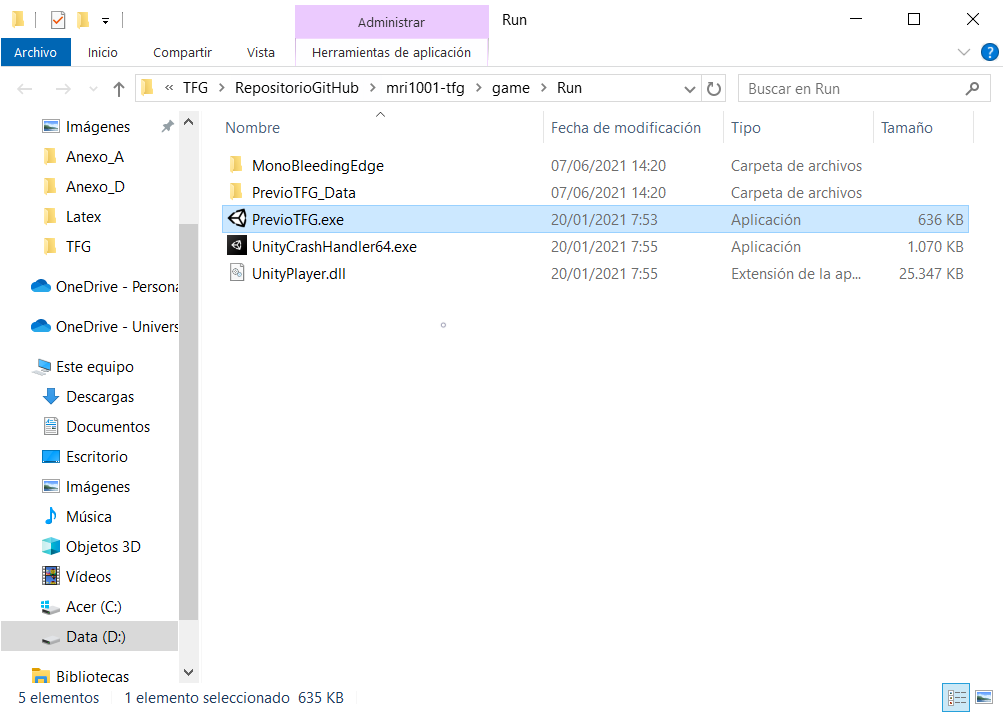
\includegraphics[scale=0.3]{Anexos/Anexo_D/Export}
\caption{Ficheros generados al exportar el juego}
\end{figure}

Entre los ficheros generados un .exe. Ese es el que iniciará la ejecución del juego.

\section{Compilación, instalación y ejecución del proyecto}

\subsection{Instalación}
Para este proyecto solo es necesario tener instalado Unity. Para descargarlo hay que acceder a la siguiente página web: \url{https://unity3d.com/get-unity/download}

\begin{figure}[h]
\centering
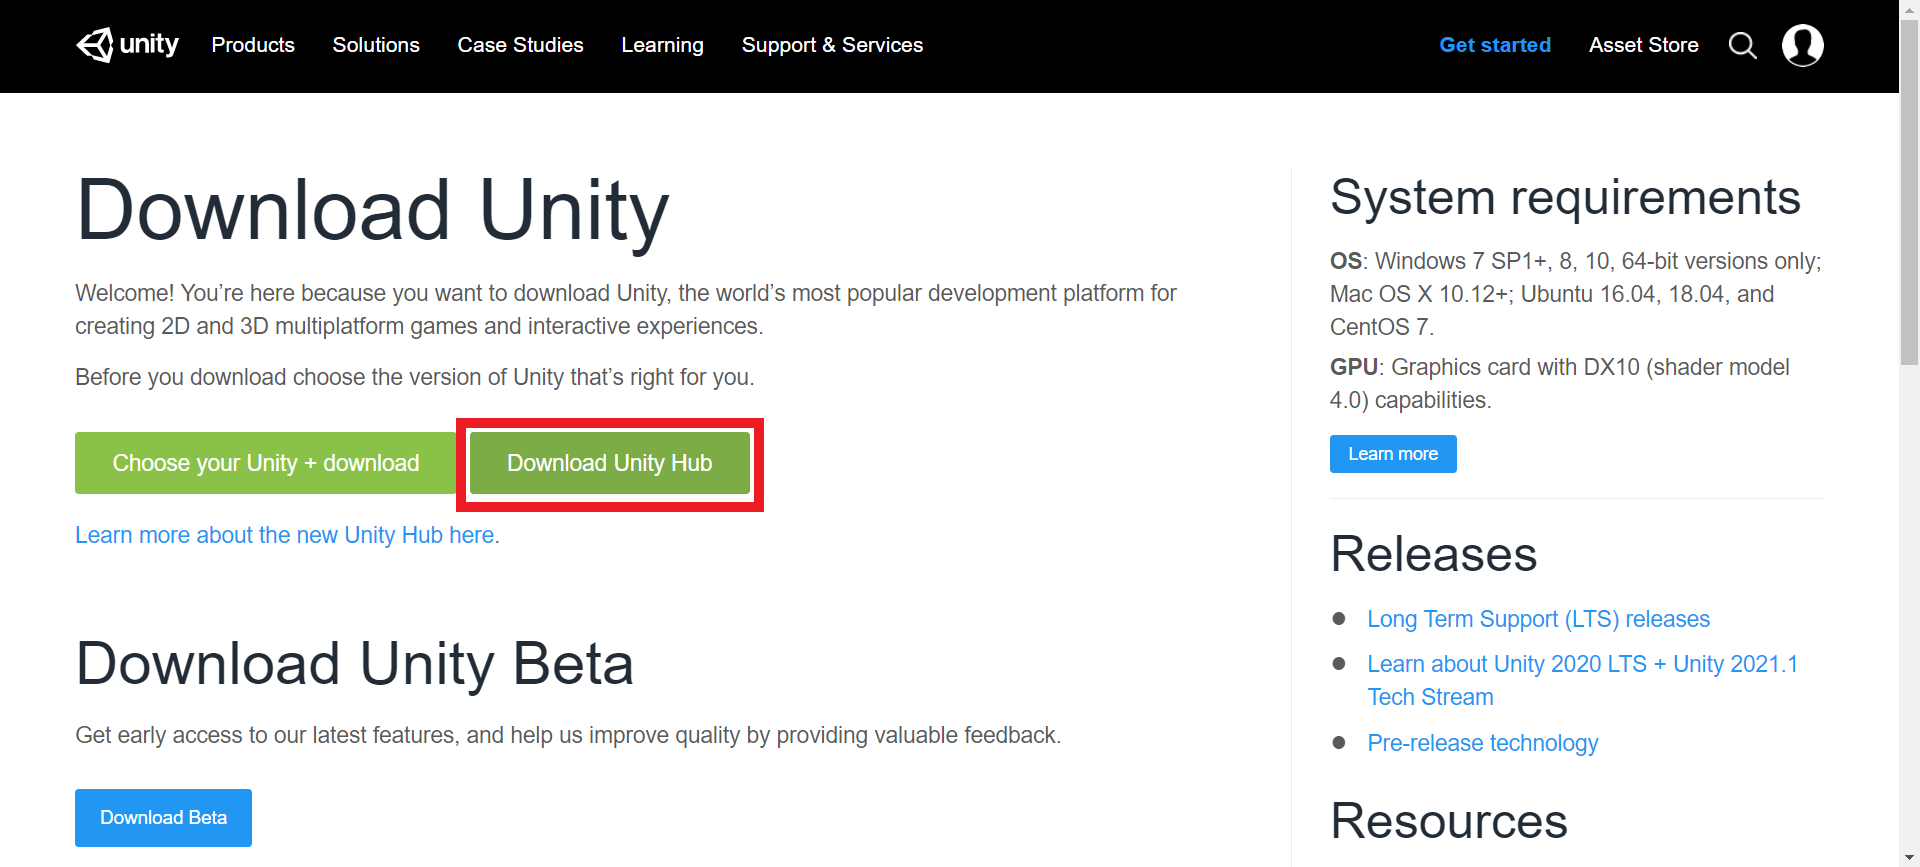
\includegraphics[scale=0.3]{Anexos/Anexo_D/Descarga_Unity}
\caption{Página de descarga de Unity}
\end{figure}

Pulsando el botón de ''Download Unity Hub'' se descargará un ejecutable. Al ejecutarlo comenzará la instalación del Unity Hub. Es una instalación normal, con seguir las instrucciones y aceptar los términos de uso el Unity Hub se instalará correctamente.\\
Ahora solo falta descargar la versión de Unity que se desea. El proyecto se ha desarrollado en la versión de Unity 2019.4.19f1. Es importante tener cuidado con la versión a instalar, porque, es cierto que las versiones posteriores permiten importar el proyecto, pero si ha pasado mucho tiempo entre versiones algo se podría deprecado y no funcionar como se espera.

Para instalar La versión de Unity que queramos hay que abrir el Unity Hub y acceder a la pestaña ''Install''.

\clearpage
\begin{figure}[h]
\centering
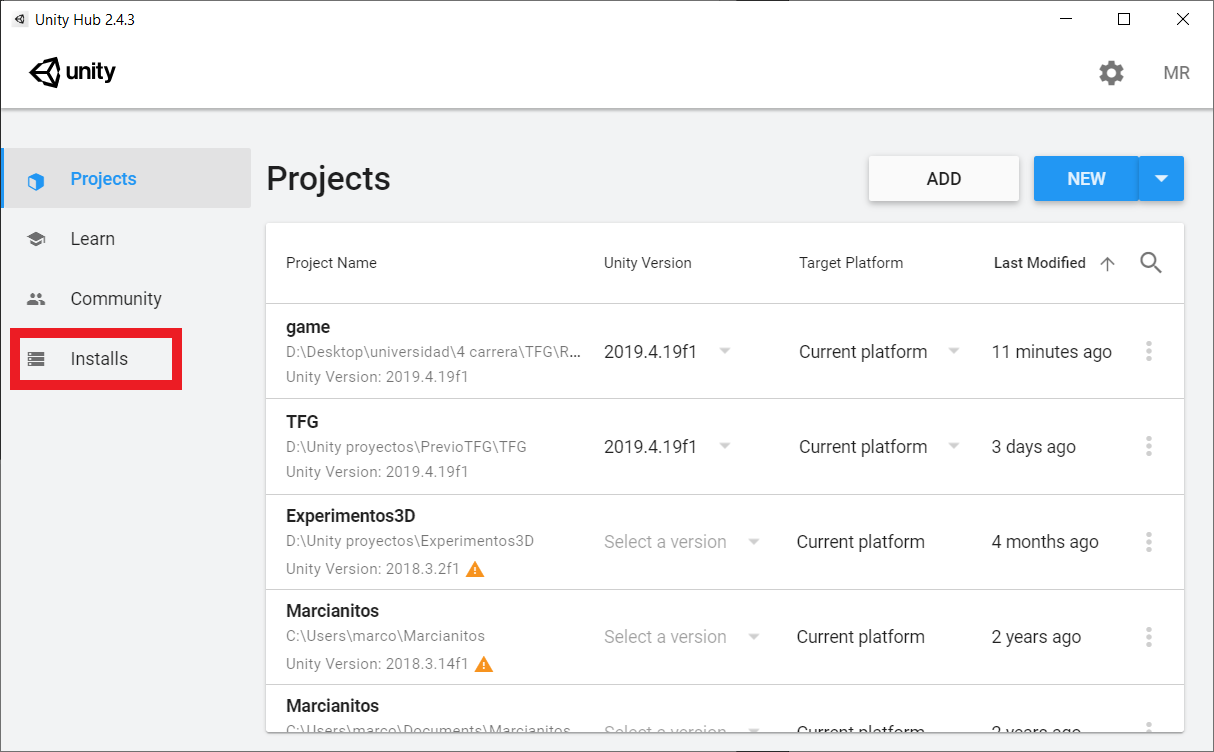
\includegraphics[scale=0.3]{Anexos/Anexo_D/UnityHub}
\caption{Unity Hub}
\end{figure}

Una vez en esa pestaña pulsar el botón de add y elegir la versión de Unity que se desea descargar.

\begin{figure}[h]
\centering
\includegraphics[scale=0.3]{Anexos/Anexo_D/UnityHub_añadir}
\caption{Descarga de una versión de Unity desde Unity Hub}
\end{figure}

\clearpage
\begin{figure}[h]
\centering
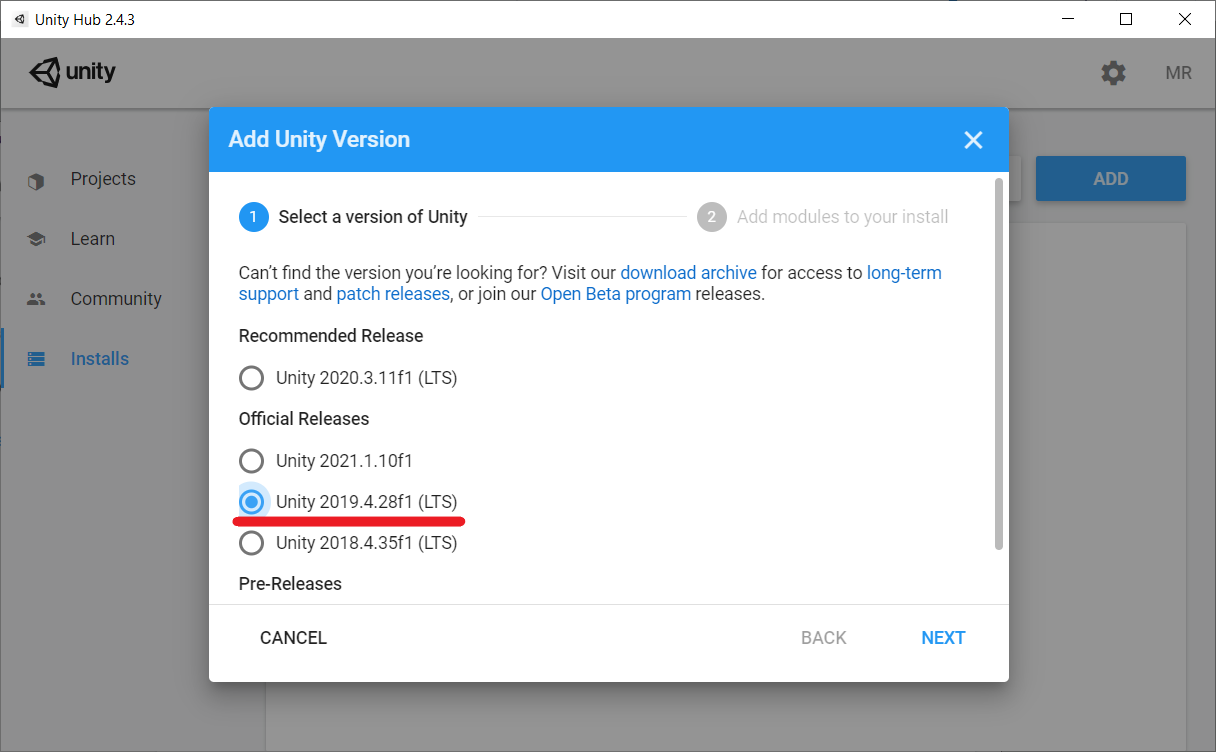
\includegraphics[scale=0.3]{Anexos/Anexo_D/UnityHub_version}
\caption{Selección de una versión de Unity desde Unity Hub}
\end{figure}

Clicando en ''Next'' aparecerán los módulos de Unity que se desean añadir a la instalación. Añadir a los que se ofrecen por defecto los módulos ''Linux Build Support (IL2CPP)'' y ''Linux Build Support (Mono)'' para que al exportar el juego también sea compatible con Linux.

\begin{figure}[h]
\centering
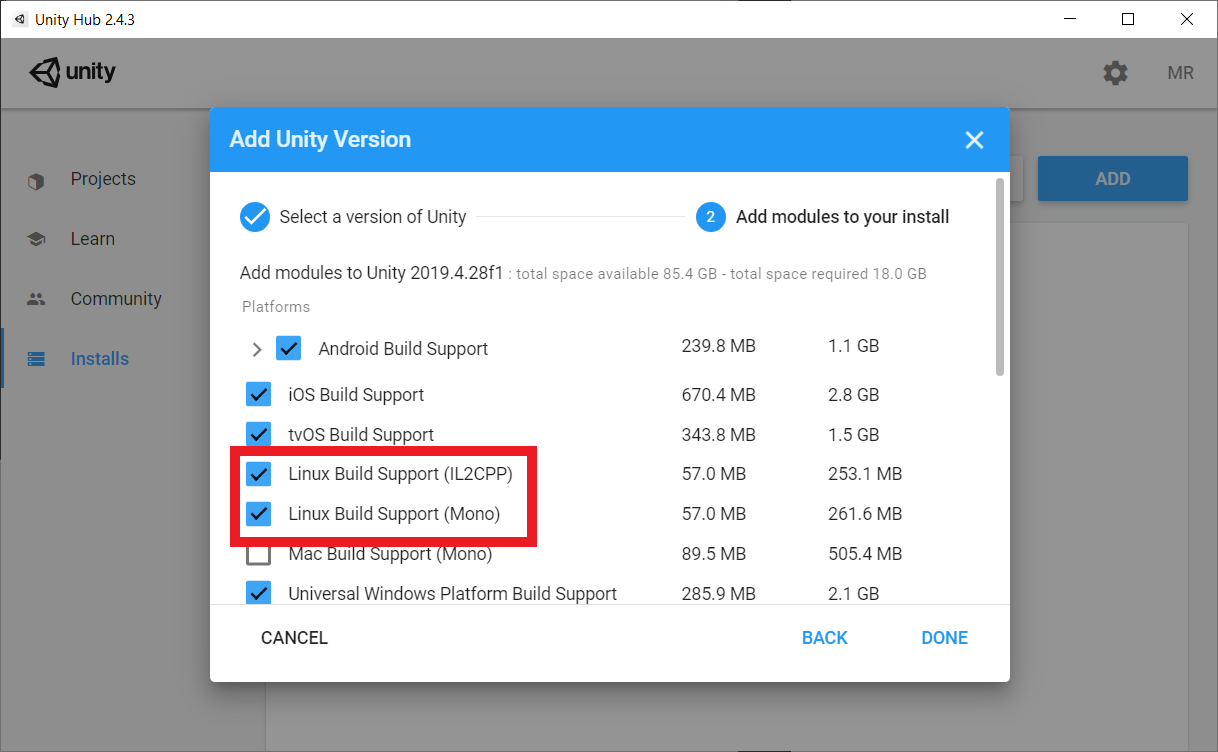
\includegraphics[scale=0.3]{Anexos/Anexo_D/UnityHub_modulos}
\caption{Selección de módulos de Unity desde Unity Hub}
\end{figure}

Pulsar en ''Next'' y esperar a que termine la instalación.

La instalación también se puede llevar a cabo después de importar el proyecto, pues no te dejará abrir el proyecto y te obligará a realizar la instalación. El proceso es similar al mostrado anteriormente. Si no se sabe la versión de Unity del proyecto que se desea importar es recomendable utilizar esta opción y descargar la versión de Unity necesaria después de importar el proyecto.

\subsection{Compilación}
Unity se compila automáticamente. Cada vez que se modifiquen los scripts utilizados en el proyecto y se vuelva a la ventana de la aplicación de Unity se guardarán los cambios y compilará el proyecto. Si surgen errores se mostrarán en la consola que ofrece Unity.
 Adicionalmente la consola de Unity añade las opciones ''Clear'' para limpiar el contenido de la consola, ''Clear on Play'' para limpiar el contenido de la consola cada vez que se ejecute el juego en el editor, ''Collapse'' para juntar los mensajes de la consola que sean iguales en solo uno, ''Clear on Build'', para limpiar el contenido de la consola cada vez que se exporte el proyecto, y ''Error pause'' para pausar la ejecución del programa cuando salte un error de ejecución.

\begin{figure}[h]
\centering
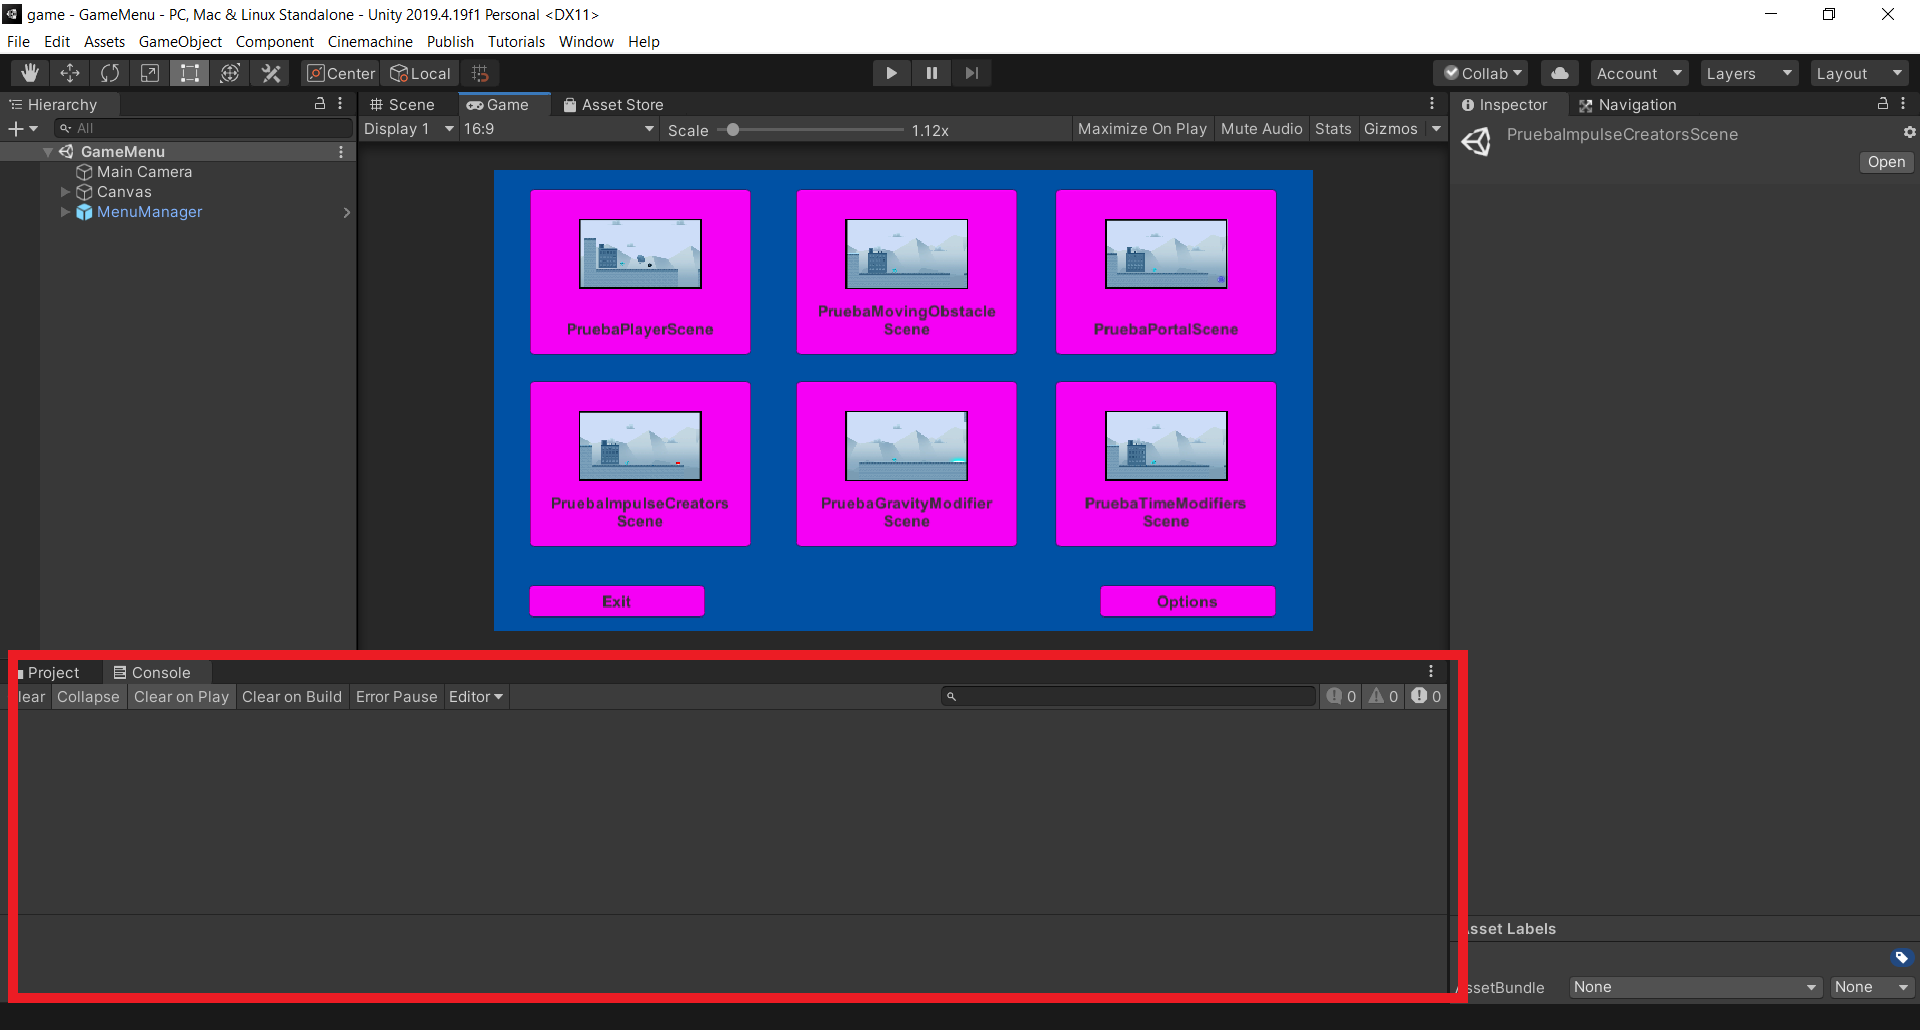
\includegraphics[scale=0.3]{Anexos/Anexo_D/Consola_Unity}
\caption{Consola de Unity}
\end{figure}

Es posible que la consola no se encuentre en esa posición exacta de la ventana de Unity, pero siempre se podrá acceder a ella a través de la pestaña de Window → Windows → Console de la barra de herramientas superior de Unity.

\subsection{Ejecución del proyecto}
El proyecto se puede ejecutar antes de exportarlo para tener una aproximación a los que será el producto exportado. Para ello se ha de pulsar el botón de ''Play'' del editor de Unity. La ejecución se parará cuando se vuelva a pulsar el botón de ''Play''. Tener en cuenta que las instrucciones de cierre del programa no funcionarán en el editor pero si en la exportación.\\
La ejecución del programa se puede pausar desde el botón de ''Pause''. Cuando se vuelva a pulsar este botón se reanudará la ejecución.

\begin{figure}[h]
\centering
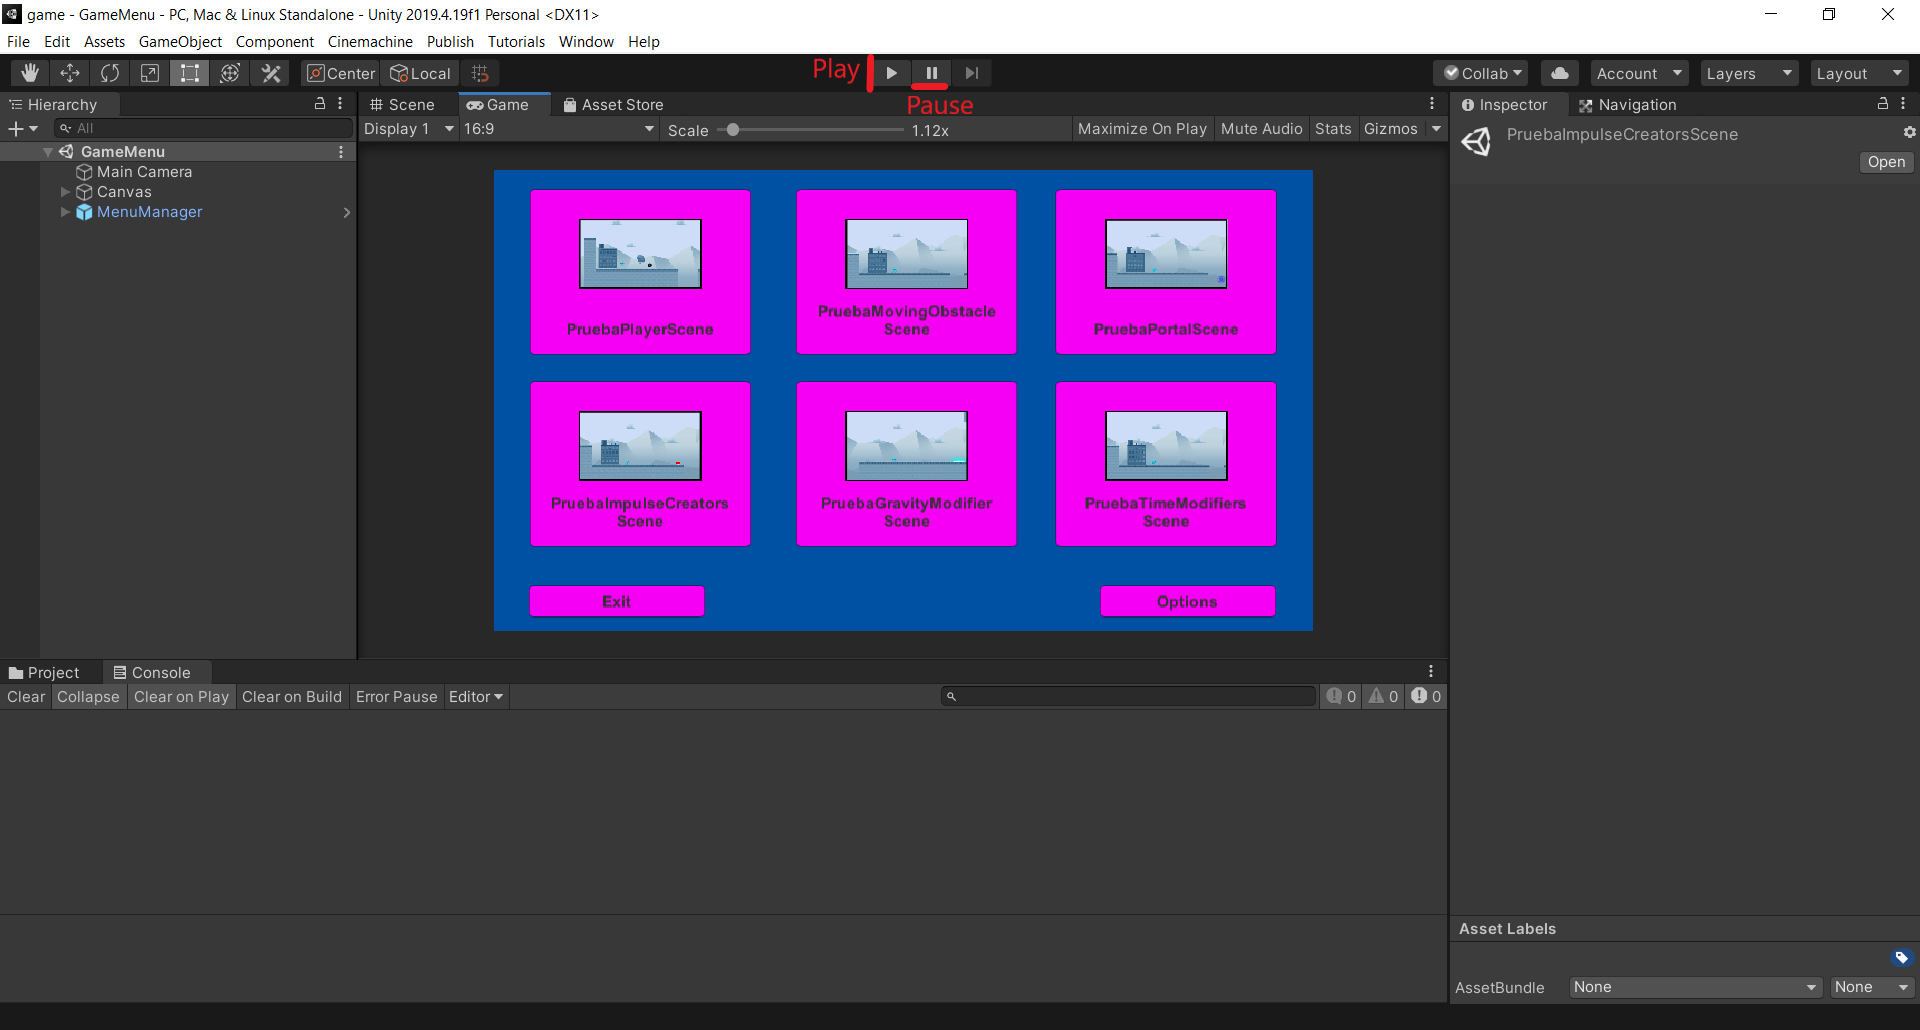
\includegraphics[scale=0.3]{Anexos/Anexo_D/Play_Pause}
\caption{Botones de ''Play'' y ''Pause'' del editor de Unity}
\end{figure}

\section{Pruebas del sistema}
Como se ha mencionado en la memoria la realización de pruebas durante el desarrollo de un videojuego es un tema complejo. Debido a ello no ha sido posible realizar pruebas automáticas. Sin embargo, se ha querido representar el funcionamiento básico de videojuego (deducido a partir de los casos de uso y el documento de diseño de juego), que si bien no sirven como sistema de pruebas, formalizan el funcionamiento esperado del programa, permitiendo comprobar si se está realizando una correcta implementación del programa o allanando en el terreno por si en el futuro fuese posible implementar pruebas automáticas.

Para este propósito se ha seguido el sistema de representación de test Given-When-Then \cite{GWT}. Este sistema de representación se sirve de tres premisas para estructurar los test:
\begin{itemize}
\item
Given: Para describir el estado del programa antes de realizar la acción que se desea probar.
\item
When: Representará la acción que se desea probar.
\item
Then: Para describir los cambios esperados tras la realización de la prueba a realizada.
\end{itemize}

Se mostrarán a continuación las representaciones de los test desarrolladas:

\subsection{Selección de niveles}
\textbf{Given:} Se está en el menú principal.

\textbf{When:} Se selecciona el nivel al que se desea viajar (PruebaPlayerScene) y se pulsa el botón de acceso.

\textbf{Then:} Se ha viajado a la escena del nivel seleccionado (PruebaPlayerScene)

\subsection{Viaje al menú de opciones}
\textbf{Given:} Se está en el menú principal.

\textbf{When:} Se selecciona el botón de Options y se pulsa.

\textbf{Then:} Se ha viajado al menú de opciones (OptionsScene)

\subsection{Modificar una opción}
\textbf{Given:} Se está en el menú principal sobre la opción de Volumen general, que tiene el valor de 100.

\textbf{When:} Mover la barra de desplazamiento lo máximo hacia la izquierda.

\textbf{Then:} El texto que marca el valor del volumen general habrá cambiado a 0. El volumen del juego será 0. Si se para la aplicación y se vuelve a correr el volumen general seguirá siendo 0.

\subsection{Abrir el menú de pausa}
\textbf{Given:} Estar en un nivel jugable (PruebaPlayerScene).

\textbf{When:} Pulsar el botón asociado a la apertura del menú de pausa.

\textbf{Then:} Se ha abierto el menú de pausa y la ejecución del nivel se habrá detenido temporalmente (Time.timeScale será 0).

\subsection{Cerrar el menú de pausa}
\textbf{Given:} Estar en un nivel jugable (PruebaPlayerScene) con el menú de opciones abierto.

\textbf{When:} Se pulsará el botón del controlador que se esté usando asociado al cierre del menú de pausa o se pulsará el botón del menú de pausa asociado con el cierre del menú de pausa.

\textbf{Then:} Se ha cerrado el menú de pausa y la ejecución del nivel se habrá retomado (Time.timeScale será 1).

\subsection{Vuelta al menú principal}
\textbf{Given:} Estar en un nivel jugable (PruebaPlayerScene) con el menú de opciones abierto.

\textbf{When:} Pulsar el botón del menú de opciones ''Back to Main Menú''.

\textbf{Then:} Se habrá pasado al menú principal.

\subsection{Invertir gravedad del Player}
\textbf{Given:} Estar en un nivel jugable con inversores de gravedad (PruebaGravityModifiersScene). El Player tiene una gravedad de Phisics2d.gravity (sin modificaciones).

\textbf{When:} El Player entra en contacto con un inversor de gravedad.

\textbf{Then:} La gravedad del Player se invierte siendo ahora -Phisics2d.gravity.

\subsection{Entrar a la zona de influencia de un obstáculo superdenso}
\textbf{Given:} Estar en un nivel jugable con un obstáculo superdenso (PruebaGravityModifiersScene). El Player tiene una gravedad de Phisics2d.gravity (sin modificaciones).

\textbf{When:} El Player entra en la zona de influencia del obstáculo superdenso.

\textbf{Then:} La gravedad del Player se modifica al entrar en la zona de influencia, aumentando en la dirección del obstáculo superdenso hasta que colisiona con este y muere.

\subsection{Entrar en una zona de modificación temporal}
\textbf{Given:} Estar en un nivel jugable con una zona de modificación temporal (PruebaTimeModifiersScene). La escala de tiempo del Player es la por defecto.

\textbf{When:} El Player se desplaza hasta entrar en la zona de modificación temporal.

\textbf{Then:} La escala de tiempo del Player pasa a ser la escala de tiempo por defecto * la modificación a la escala temporal de la zona de modificación temporal.

\subsection{Salir de una zona de modificación temporal}
\textbf{Given:} Estar en un nivel jugable con una zona de modificación temporal (PruebaTimeModifiersScene). El Player se encuentra en una zona de modificación temporal. La escala de tiempo del Player es la por defecto * la modificación a la escala temporal de la zona de modificación temporal.

\textbf{When:} El Player se desplaza hasta salir de la zona de tiempo invertido.

\textbf{Then:} La escala de tiempo del Player pasa a ser la escala que tenía / la modificación a la escala temporal de la zona de modificación temporal (la escala de tiempo por defecto).

\subsection{Modificar el tiempo a nivel global}
\textbf{Given:} Estar en un nivel jugable (PruebaPlayerScene).

\textbf{When:} Pulsar el botón asociado a la mecánica de tiempo bala del Player.

\textbf{Then:} La ejecución del nivel se reducirá (Time.timescale se reducirá) y pasado un tiempo volverá a su estado natural (Time.timescale = 1)

\subsection{Utilizar una plataforma de salto}
\textbf{Given:} Estar en un nivel jugable con una plataforma de salto (PruebaImpulseCreatorsScene).

\textbf{When:} El Player entra en contacto con la plataforma de salto.

\textbf{Then:} El Player sale impulsado hacia arriba. Su velocidad (la RigidBody2D.Velocity del Player) habrá variado en el eje de las Y, pero no en el de las X. RigidBody2D.Velocity.Y del Player será ahora RigidBody2D.Velocity.Y + impulso de la plataforma de salto. RigidBody2D.Velocity.X deberá seguir siendo la misma.

\subsection{Utilizar una partícula de impulso}
\textbf{Given:} Estar en un nivel jugable con una partícula de impulso (PruebaImpulseCreatorsScene).

\textbf{When:} El Player entra en contacto con la partícula de impulso.

\textbf{Then:} El Player sale impulsado en la dirección designada por la partícula de impulso. RigidBody2D.Velocity.Y del Player será ahora RigidBody2D.Velocity.Y + impulso de la partícula de impulso en el eje de las Y. RigidBody2D.Velocity.X deberá ser RigidBody2D.Velocity.X + impulso de la partícula de impulso en el eje de las X.

\subsection{Utilizar un amplificador de impulso}
\textbf{Given:} Estar en un nivel jugable con un amplificador de impulso (PruebaImpulseCreatorsScene).

\textbf{When:} El Player entra en contacto con el amplificador de impulso.

\textbf{Then:} La velocidad del Player se escalará en la cantidad designada por el amplificador de impulso. RigidBody2D.Velocity del Player será ahora RigidBody2D.Velocity * multiplicador del amplificador de impulso.

\subsection{Colisionar con una pared}
\textbf{Given:} Estar en un nivel jugable con paredes (PruebaPlayerScene). El Player lleva una velocidad de 6 en el eje de las X y -3 en el de las Y.

\textbf{When:} El Player colisiona con una pared a su derecha (la dirección en el eje de las X en el que se está desplazando).

\textbf{Then:} El Player debe estar al lado de la pared. La velocidad en la dirección del muro debe cesar pero el resto continuar. La velocidad del Player será ahora 0 en el eje de las X y -3 en el eje de las Y.

\subsection{Colisionar con el suelo}
\textbf{Given:} Estar en un nivel jugable con suelos (PruebaPlayerScene). El Player lleva una velocidad de 6 en el eje de las X y -3 en el de las Y.

\textbf{When:} El Player colisiona con el suelo que hay a sus pies (la dirección en el eje de las Y en el que se está desplazando).

\textbf{Then:} El Player debe estar encima del suelo. La velocidad en la dirección del suelo debe cesar pero el resto continuar. La velocidad del Player será ahora 6 en el eje de las X y 0 en el eje de las Y.

\subsection{Entrar por un portal}
\textbf{Given:} Estar en un nivel jugable con un par de portales enlazados (portal1 y portal2) (PruebaPortalesScene).

\textbf{When:} El Player entra por el portal1.

\textbf{Then:} El Player se habrá teletransportando pasando a ser su nueva posición la del portal2.

\subsection{Mover al Player a la derecha}
\textbf{Given:} Estar en un nivel jugable con un Player (PruebaPlayerScene).

\textbf{When:} El Player pulsa el botón de desplazamiento hacia la derecha.

\textbf{Then:} La velocidad del Player habrá aumentado en el eje de las X positivamente. El Player se habrá desplazado hacia la derecha.

\subsection{Mover al Player a la izquierda}
\textbf{Given:} Estar en un nivel jugable con un Player (PruebaPlayerScene).

\textbf{When:} El Player pulsa el botón de desplazamiento hacia la izquierda.

\textbf{Then:} La velocidad del Player habrá disminuido en el eje de las X. El Player se habrá desplazado hacia la izquierda.

\subsection{Saltar con el Player}
\textbf{Given:} Estar en un nivel jugable con un Player (PruebaPlayerScene).

\textbf{When:} El Player pulsa el botón de salto.

\textbf{Then:} La velocidad del Player habrá aumentado en el eje de las Y. El Player realizará el salto.

\subsection{Realizar el acelerón con el Player}
\textbf{Given:} Estar en un nivel jugable con un Player (PruebaPlayerScene).

\textbf{When:} El Player pulsa el botón del acelerón.

\textbf{Then:} La velocidad del Player pasará a ser constante siendo 0 en el eje de las Y, y +(velocidad del aceleron) en el eje de las X en caso de haber estado yendo hacia la derecha o -(velocidad del aceleron) en el eje de las X en caso de haber estado yendo hacia la izquierda. El Player realizará el salto.

\subsection{Muerte contra un obstáculo}
\textbf{Given:} Estar en un nivel jugable con obstáculos (PruebaPlayerScene).

\textbf{When:} El Player colisiona con el obstáculo.

\textbf{Then:} Se debe iniciar la cadena de eventos de muerte del Player.

\subsection{Cadena de eventos de la muerte del Player}
\textbf{Given:}Estar en un nivel jugable (PruebaPlayerScene).

\textbf{When:} El Player muere.

\textbf{Then:} Se destruyen los objetos instanciados durante la ejecución el nivel y se reinicia el nivel devolviéndolo al estado inicial.

\subsection{El Player cae en una zona de muerte}
\textbf{Given:} Estar en un nivel jugable con zonas de muerte (PruebaPlayerScene).

\textbf{When:} El Player colisiona con la zona de muerte.

\textbf{Then:} Se debe iniciar la cadena de eventos de muerte del Player.

\subsection{El Player cae en una zona de victoria}
\textbf{Given:} Estar en un nivel jugable con zonas de victoria (PruebaPlayerScene).

\textbf{When:} El Player colisiona con la zona de victoria.

\textbf{Then:} El Player realiza la animación de llegada a la zona de victoria y se transiciona al menú principal.

\subsection{El obstáculo que sigue una rutina se mueve}
\textbf{Given:} Estar en un nivel jugable con un obstáculo que sigue una rutina (PruebaPlayerScene).

\textbf{When:} Pasar loops de ejecución del programa.

\textbf{Then:} El obstáculo debe haber pasado por todos los puntos que componen su rutina de viaje y haber vuelto a la posición inicial. Al haber vuelto a la posición inicial se debe continuar el movimiento del obstáculo repitiendo la rutina del viaje hasta que se pare la ejecución.

\subsection{El obstáculo móvil se mueve}
\textbf{Given:} Estar en un nivel jugable con un obstáculo que sigue una rutina (PruebaMovingObstacleScene).

\textbf{When:} Pasar loops de ejecución del programa.

\textbf{Then:} El obstáculo móvil tiene que avanzar de derecha a izquierda indefinidamente. Su posición en el eje de las X tiene que ser siempre menor que la que llevaba anteriormente.